\section{Atividades}

\subsection{Entrega da Atividade}

\paragraph{}
Como evidência da conclusão deste roteiro foi solicitada uma captura de tela
demonstrando que o usuário \texttt{user} conseguiu obter privilégios elevados
no sistema.

\paragraph{}
Para validação da atividade foi utilizado o comando:

\begin{verbatim}
net user user
\end{verbatim}

\paragraph{}
A comprovação foi realizada observando a associação do usuário ao grupo
\texttt{Administrators}, evidenciando o sucesso da escalação de privilégios.

\begin{figure}[H]
  \centering
  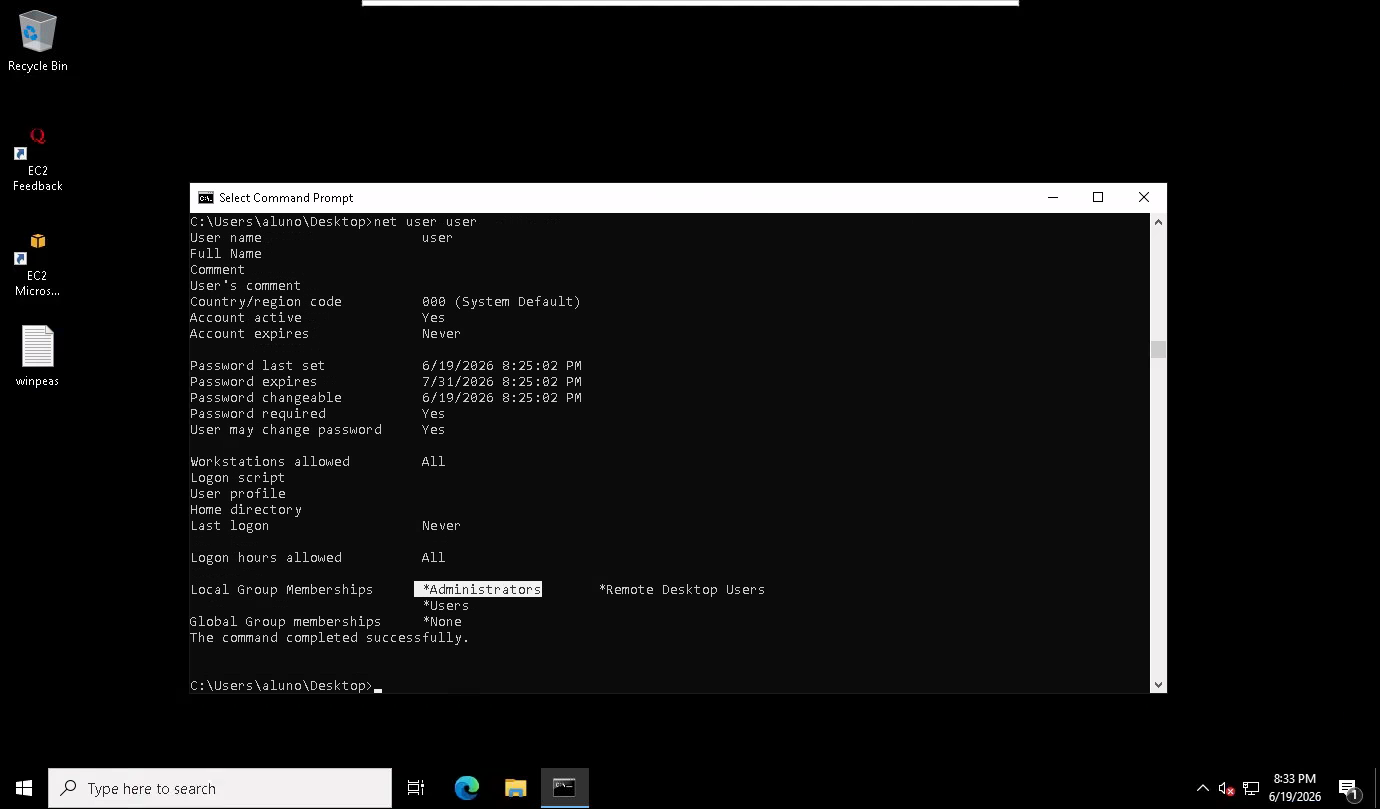
\includegraphics[width=0.9\textwidth]{./fig/atividade-entrega.png}
  \caption{Comprovação da escalação de privilégios do usuário \texttt{user}.}
\end{figure}

\subsection{Preparação do Ambiente}

\paragraph{}
Antes da execução das atividades foi realizada a preparação do ambiente de
laboratório utilizando uma conta com privilégios administrativos.

\paragraph{}
Foram modificadas políticas de senha do sistema para simplificar a criação de
contas utilizadas durante os testes, além da criação de usuários locais e da
configuração de permissões necessárias para acesso remoto.

\paragraph{}
Também foram geradas cópias de segurança dos arquivos \texttt{SAM} e
\texttt{SYSTEM}, armazenadas em diretórios acessíveis para posterior utilização
nas atividades relacionadas à recuperação e quebra de credenciais.

\subsection{Atividade 1 -- Ferramentas de Enumeração}

\paragraph{}
Nesta atividade foram utilizadas ferramentas automatizadas de enumeração com o
objetivo de coletar informações relevantes sobre o sistema operacional Windows.

\paragraph{}
A ferramenta \texttt{WinPEAS} foi executada para realizar uma análise completa
do ambiente, produzindo um relatório contendo informações sobre usuários,
grupos, serviços, permissões, registros, tarefas agendadas e potenciais vetores
de escalação de privilégios.

\paragraph{}
O relatório gerado foi salvo em arquivo para permitir consultas posteriores e
análises mais detalhadas das informações coletadas.

\paragraph{}
Também foram exploradas diferentes formas de visualização do relatório,
incluindo leitura diretamente pelo Prompt de Comando e transferência do arquivo
para a máquina atacante para análise em ferramentas mais adequadas.

\paragraph{}
A atividade permitiu compreender a importância de ferramentas automatizadas para
reduzir erros operacionais e acelerar o processo de enumeração durante testes de
segurança.

\subsection{Atividade 2 -- Serviço com Permissão Fraca}

\paragraph{}
Nesta prática foi explorada uma vulnerabilidade relacionada a permissões
inadequadas aplicadas sobre um serviço do Windows.

\paragraph{}
Através das informações identificadas pela ferramenta \texttt{WinPEAS} foi
possível verificar que o serviço permitia alterações em sua configuração por um
usuário sem privilégios administrativos.

\paragraph{}
Utilizando ferramentas nativas do sistema foram analisadas as permissões do
serviço e identificado o programa configurado para execução.

\paragraph{}
Posteriormente a configuração do serviço foi modificada para executar um comando
responsável por adicionar o usuário \texttt{user} ao grupo
\texttt{Administrators}.

\paragraph{}
Após a inicialização do serviço foi possível verificar que o comando foi
executado com sucesso e que o usuário passou a possuir privilégios
administrativos no sistema.

\paragraph{}
Ao final da atividade o usuário foi removido do grupo administrativo para que o
ambiente permanecesse consistente para as próximas etapas do roteiro.

\subsection{Atividade 3 -- Serviço com Caminho sem Aspas}

\paragraph{}
Nesta atividade foi explorada uma vulnerabilidade conhecida como
\textit{Unquoted Service Path}.

\paragraph{}
Foi realizada a análise da configuração de um serviço cujo caminho do executável
estava definido sem aspas, permitindo que o sistema operacional interpretasse
incorretamente o caminho durante o processo de inicialização.

\paragraph{}
Com base nesse comportamento foi criado um executável compatível com serviços do
Windows contendo um comando responsável por adicionar o usuário
\texttt{user} ao grupo \texttt{Administrators}.

\paragraph{}
O executável foi posicionado em um dos caminhos que o Windows tenta executar
antes de alcançar o binário originalmente configurado pelo serviço.

\paragraph{}
Após a inicialização do serviço foi possível confirmar que o executável criado
foi executado e que o usuário recebeu privilégios administrativos.

\paragraph{}
Ao término dos testes a associação do usuário ao grupo administrativo foi
removida para manter a consistência do ambiente.

\subsection{Atividade 4 -- Injeção de DLL}

\paragraph{}
Nesta etapa foi explorada uma técnica de \textit{DLL Hijacking}, baseada na
ausência de bibliotecas dinâmicas necessárias para execução de um serviço do
Windows.

\paragraph{}
Utilizando o \texttt{Process Monitor (ProcMon)} foi possível identificar as
tentativas de carregamento de uma DLL inexistente realizadas pelo serviço.

\paragraph{}
Após a identificação do local pesquisado pelo sistema, foi criada uma DLL
maliciosa contendo um comando responsável por adicionar o usuário
\texttt{user} ao grupo \texttt{Administrators}.

\paragraph{}
A biblioteca foi compilada utilizando o ambiente \texttt{MinGW} e posicionada
no diretório esperado pelo serviço.

\paragraph{}
Quando o serviço foi iniciado, a DLL criada foi carregada automaticamente,
executando o código definido e concedendo privilégios administrativos ao
usuário.

\paragraph{}
Concluídos os testes, o usuário foi removido do grupo administrativo para
prosseguimento das demais atividades.

\subsection{Atividade 5 -- Quebra de Senhas}

\paragraph{}
A última atividade teve como objetivo explorar o acesso a cópias de segurança
dos arquivos \texttt{SAM} e \texttt{SYSTEM} do Windows para recuperação de
credenciais.

\paragraph{}
Os arquivos foram transferidos da máquina Windows para a máquina atacante por
meio de um servidor de transferência de arquivos temporário.

\paragraph{}
Com posse dos arquivos foi utilizada a ferramenta \texttt{pwdump} para extrair
as hashes de autenticação armazenadas pelo sistema operacional.

\paragraph{}
As hashes obtidas foram então processadas pela ferramenta \texttt{John the
Ripper}, permitindo a tentativa de recuperação das senhas através de ataques de
quebra de hashes.

\paragraph{}
A atividade demonstrou como o simples acesso aos arquivos de autenticação do
Windows pode permitir a obtenção de credenciais válidas e, consequentemente, o
comprometimento de contas existentes no sistema.

\paragraph{}
Além disso, foram discutidas alternativas como o uso do \texttt{Hashcat} para
realizar ataques de recuperação de senhas utilizando diferentes estratégias de
quebra de hashes.
